Fermi liquid theory only holds if the ground state of the interacting
system is connected adiabatically to the non-interacting Fermi sea. One can treat this
as turning on the interactions adiabatically. The ground state $\gs$ of the full system and
the excitation state $\blue{\ket{\vc{k}, \sigma}}$ can then be written as
\begin{equation*}
	\gs = U \ket{\Omega},
	\hspace{10 mm} 
	\blue{\ket{\vc{k}, \sigma}} = U \ket{\vc{k}, \sigma} = U c\D_{\vc{k},\sigma} \ket{\Omega}.
\end{equation*}
The time evolution operator in the interaction picture can be
expressed as a time-ordered exponential
\begin{equation*}
	U = T\left\{
		e^{- i \int_{-\infty}^{0} \hat{V}(t) \d t}
	\right\}.
\end{equation*}
The quasi-particle creation operator (№3) could be expressed from the 
\begin{equation*}
	\blue{\ket{\vc{k}, \sigma}} = a\D_{\vc{k}, \sigma} \gs = U c\D_{\vc{k}, \sigma} \ket{\Omega} = U c\D_{\vc{k}, \sigma} U^{-1} \ket{\varphi},
	\hspace{0.5cm} \Rightarrow \hspace{0.5cm}
	a\D_{\vc{k}, \sigma} = U c\D_{\vc{k}, \sigma} U^{-1}.
\end{equation*}

For Fermi liquid theory to be valid, one need to add requirement on
the wavefunction renormalization constant
\begin{equation*}
	Z_k = |\bk{\blue{k \sigma}}[c\D_{k \sigma}]{\text{gs}}|^2 = |\bk{\text{gs}}[a_{k\sigma} c\D_{k \sigma}]{\text{gs}}|^2 .
\end{equation*}
Expressing $c\D_{k \sigma}$ as a series in the quasi-particle operators
\begin{align*}
	c\D_{k \sigma} &= U\D a\D_{k \sigma} U \approx \left(
		1 + i \int_{-\infty}^{0} \hat{V}(t) \d t
	\right) a\D_{k \sigma} \left(1 - i \int_{-\infty}^{0} \hat{V}(t) \d t\right) = a\D_{k \sigma} + i \int_{-\infty}^{0} [\hat{V}(t), a\D_{k\sigma}] \d t + O(V^2) \\
	&= \sqrt{Z_k} a\D_{k \sigma} + \text{higher order}
\end{align*}
If we want to $c_{k \sigma}\D \approx a_{k \sigma}\D$, then (№4) $0 < \sqrt{Z_k} < 1$.


The spectral function (fig. \ref{fig:Apeak})
\begin{equation*}
	A(k, \omega) = - \frac{1}{\pi} \Im G^{\text{ret}} (k, \omega) = \sum_\lambda |M_\lambda|^2 \delta(\omega-\xi_\lambda),
	\hspace{10 mm} 
	|M_\lambda|^2 = |\bk{\lambda}[c\D_{k, \sigma}]{\text{gs}}|^2
\end{equation*}
exhibits a sharp quasiparticle peak at $\xi_k$
\begin{equation*}
	A(k, \omega) = Z_k \delta(\omega - \xi_k) + \ldots
\end{equation*}
with $Z_k > 0$. Thus momentum distribution $\langle \hat{n}_{k \sigma}\rangle$  has a jump at the Fermi momentum
\begin{equation*}
	\langle \hat{n}_{k \sigma}\rangle = \bk{\text{gs}}[c\D_{k \sigma} c_{k \sigma}]{\text{gs}} =
 \int A(k, \omega) n_f(k, \omega) \d \omega = \int Z_k \delta(\omega-\varepsilon_k) \theta(\varepsilon_f - \theta)  \d \omega + \ldots 
	= Z_k \theta(\varepsilon_F - \varepsilon_k) + \ldots
\end{equation*}

\begin{figure}[h]
    \centering
    \addletter{60}{a} 
    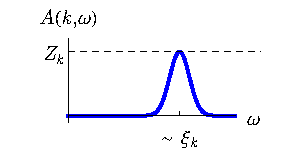
\includegraphics{imgs/Apeak.pdf}
    \hspace{10 mm} 
    \addletter{60}{b} 
    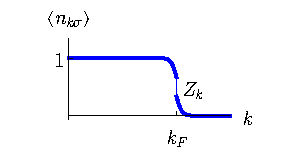
\includegraphics{imgs/npeak.pdf}
    \caption{a) The spectral function. b) The momentum distribution.}
    \label{fig:Apeak}
\end{figure}
